\artigotrue
\chapter{Título do Primeiro artigo}
\label{chap:chapter01}

\begin{chapterabstractPOR}{Palavra-chave 1, Palavra-chave 2, Palavra-chave 3}
\noindent{Este é o resumo do primeiro artigo da tese.}
\end{chapterabstractPOR}

\begin{chapterabstractENG}{Key-word 1. Key-word 2. Key-word 3}
\noindent{This is the abstract of the first article of the thesis.}
\end{chapterabstractENG}

\section{INTRODUÇÃO}

\blindtext[2]

\section{MATERIAL E MÉTODOS}

Este é um texto bem formatado, escrito em Seropédica, RJ. \blindtext[1]

Este é o código fote de uma função construída no ambiente R:

\begin{verbatim}
> soma <- function (a, b) {a + b}
> soma(2, 2)
[1] 4
\end{verbatim}

Está é uma matriz bem formatada:

\begin{equation}
  A_{m,n} =
 \begin{pmatrix}
  a_{1,1} & a_{1,2} & \cdots & a_{1,n} \\
  a_{2,1} & a_{2,2} & \cdots & a_{2,n} \\
  \vdots  & \vdots  & \ddots & \vdots  \\
  a_{m,1} & a_{m,2} & \cdots & a_{m,n}
 \end{pmatrix}
\end{equation}

\begin{subequations}\label{eq:maxwell}
E estas são as equações de Maxwell:
\begin{align}
        B'&=-\nabla \times E,\\
        E'&=\nabla \times B - 4\pi j,
\end{align}
\end{subequations}

\section{RESUTADOS}

Aqui está mais um texto bem formatado. \blindtext[1]

Que tal fazer um link para a figura \autoref{fig:ocio}? E também citar o \citet{Feyerabend1977} com um link para a localização da referência bibliográfica?

\begin{figure}[!ht]
\centering
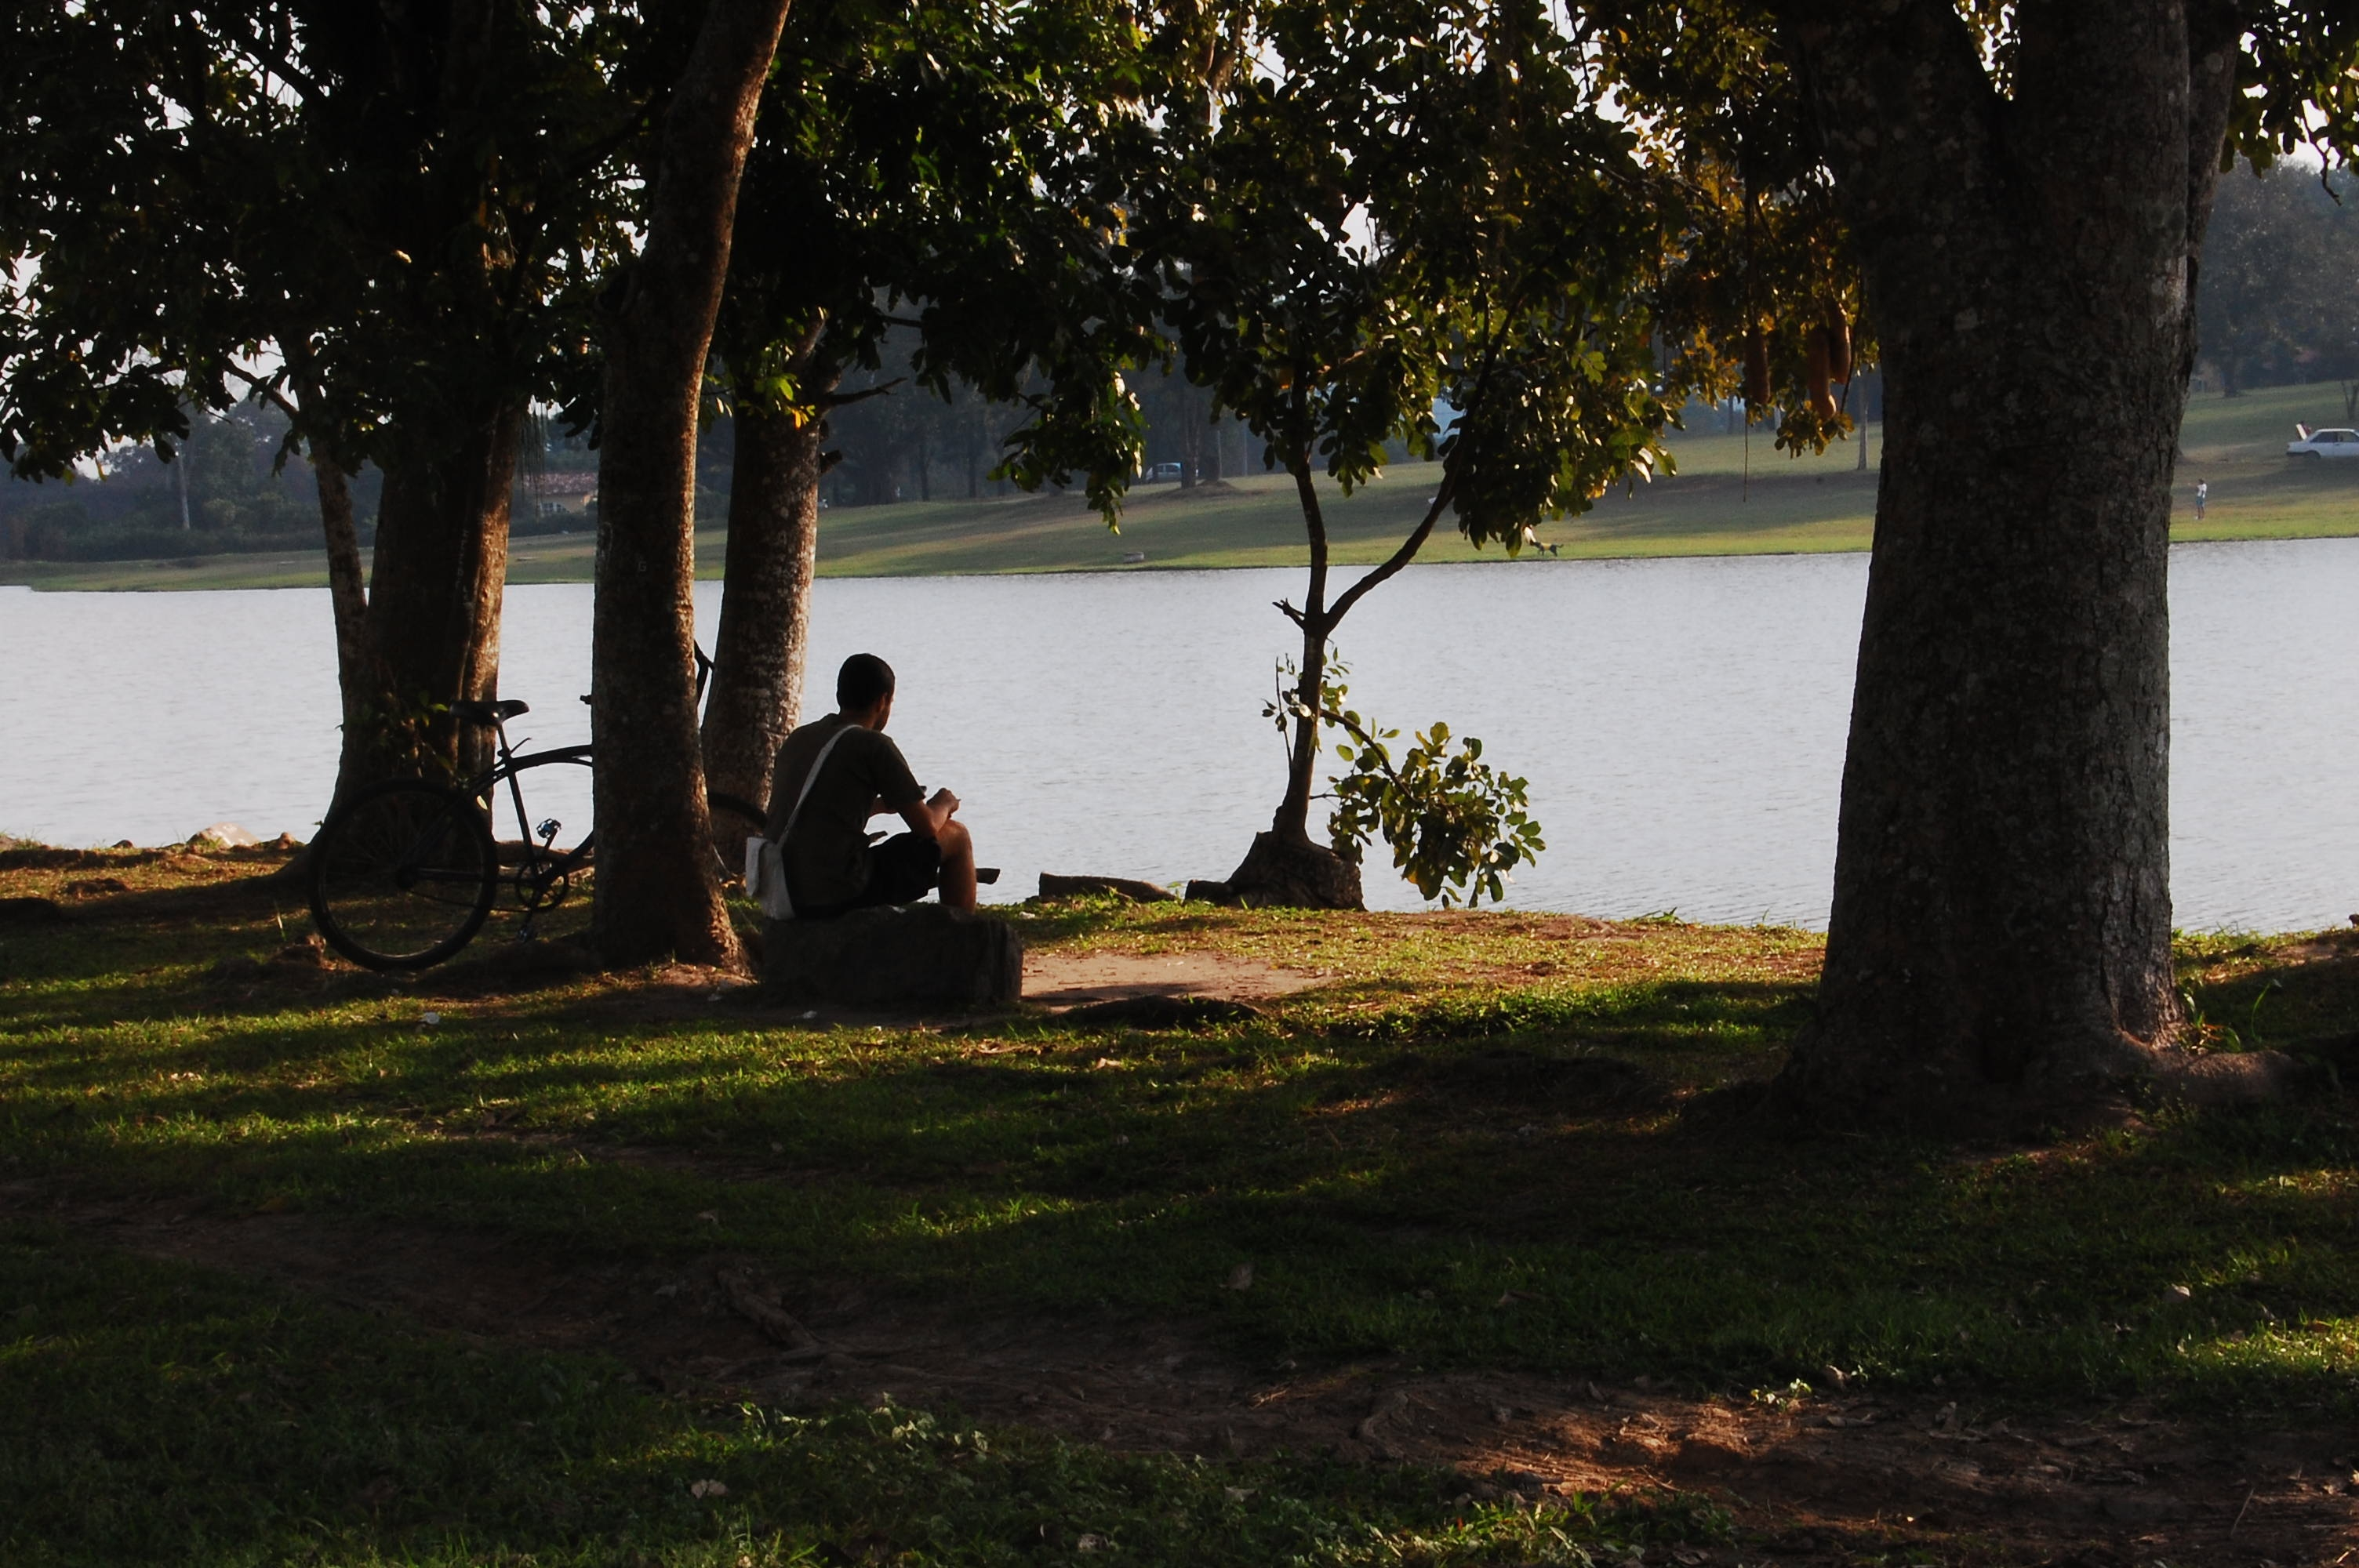
\includegraphics[width=16cm]{figura02}
\caption{\label{fig:ocio}O ócio criativo. Fonte: \url{http://r1.ufrrj.br/graduacao/img/acesso-2012/o-ocio-criativo.jpg}}
\end{figure}

\section{DISCUSSÃO}

Aqui está o último texto muito bem formatado. \blindtext[2]

Que tal fazer um link para a equação \autoref{eq:maxwell}?

\section{CONCLUSÕES}

\begin{itemize}
  \item Está é uma conclusão importante.
  \item Está é outra conclusão importante.
  \item Está é uma conclusão menos importante.
\end{itemize}
